% Options for packages loaded elsewhere
\PassOptionsToPackage{unicode}{hyperref}
\PassOptionsToPackage{hyphens}{url}
%
\documentclass[
]{book}
\usepackage{lmodern}
\usepackage{amsmath}
\usepackage{ifxetex,ifluatex}
\ifnum 0\ifxetex 1\fi\ifluatex 1\fi=0 % if pdftex
  \usepackage[T1]{fontenc}
  \usepackage[utf8]{inputenc}
  \usepackage{textcomp} % provide euro and other symbols
  \usepackage{amssymb}
\else % if luatex or xetex
  \usepackage{unicode-math}
  \defaultfontfeatures{Scale=MatchLowercase}
  \defaultfontfeatures[\rmfamily]{Ligatures=TeX,Scale=1}
\fi
% Use upquote if available, for straight quotes in verbatim environments
\IfFileExists{upquote.sty}{\usepackage{upquote}}{}
\IfFileExists{microtype.sty}{% use microtype if available
  \usepackage[]{microtype}
  \UseMicrotypeSet[protrusion]{basicmath} % disable protrusion for tt fonts
}{}
\makeatletter
\@ifundefined{KOMAClassName}{% if non-KOMA class
  \IfFileExists{parskip.sty}{%
    \usepackage{parskip}
  }{% else
    \setlength{\parindent}{0pt}
    \setlength{\parskip}{6pt plus 2pt minus 1pt}}
}{% if KOMA class
  \KOMAoptions{parskip=half}}
\makeatother
\usepackage{xcolor}
\IfFileExists{xurl.sty}{\usepackage{xurl}}{} % add URL line breaks if available
\IfFileExists{bookmark.sty}{\usepackage{bookmark}}{\usepackage{hyperref}}
\hypersetup{
  pdftitle={Pattends and Trends -- checking},
  pdfauthor={bako},
  hidelinks,
  pdfcreator={LaTeX via pandoc}}
\urlstyle{same} % disable monospaced font for URLs
\usepackage{color}
\usepackage{fancyvrb}
\newcommand{\VerbBar}{|}
\newcommand{\VERB}{\Verb[commandchars=\\\{\}]}
\DefineVerbatimEnvironment{Highlighting}{Verbatim}{commandchars=\\\{\}}
% Add ',fontsize=\small' for more characters per line
\usepackage{framed}
\definecolor{shadecolor}{RGB}{248,248,248}
\newenvironment{Shaded}{\begin{snugshade}}{\end{snugshade}}
\newcommand{\AlertTok}[1]{\textcolor[rgb]{0.94,0.16,0.16}{#1}}
\newcommand{\AnnotationTok}[1]{\textcolor[rgb]{0.56,0.35,0.01}{\textbf{\textit{#1}}}}
\newcommand{\AttributeTok}[1]{\textcolor[rgb]{0.77,0.63,0.00}{#1}}
\newcommand{\BaseNTok}[1]{\textcolor[rgb]{0.00,0.00,0.81}{#1}}
\newcommand{\BuiltInTok}[1]{#1}
\newcommand{\CharTok}[1]{\textcolor[rgb]{0.31,0.60,0.02}{#1}}
\newcommand{\CommentTok}[1]{\textcolor[rgb]{0.56,0.35,0.01}{\textit{#1}}}
\newcommand{\CommentVarTok}[1]{\textcolor[rgb]{0.56,0.35,0.01}{\textbf{\textit{#1}}}}
\newcommand{\ConstantTok}[1]{\textcolor[rgb]{0.00,0.00,0.00}{#1}}
\newcommand{\ControlFlowTok}[1]{\textcolor[rgb]{0.13,0.29,0.53}{\textbf{#1}}}
\newcommand{\DataTypeTok}[1]{\textcolor[rgb]{0.13,0.29,0.53}{#1}}
\newcommand{\DecValTok}[1]{\textcolor[rgb]{0.00,0.00,0.81}{#1}}
\newcommand{\DocumentationTok}[1]{\textcolor[rgb]{0.56,0.35,0.01}{\textbf{\textit{#1}}}}
\newcommand{\ErrorTok}[1]{\textcolor[rgb]{0.64,0.00,0.00}{\textbf{#1}}}
\newcommand{\ExtensionTok}[1]{#1}
\newcommand{\FloatTok}[1]{\textcolor[rgb]{0.00,0.00,0.81}{#1}}
\newcommand{\FunctionTok}[1]{\textcolor[rgb]{0.00,0.00,0.00}{#1}}
\newcommand{\ImportTok}[1]{#1}
\newcommand{\InformationTok}[1]{\textcolor[rgb]{0.56,0.35,0.01}{\textbf{\textit{#1}}}}
\newcommand{\KeywordTok}[1]{\textcolor[rgb]{0.13,0.29,0.53}{\textbf{#1}}}
\newcommand{\NormalTok}[1]{#1}
\newcommand{\OperatorTok}[1]{\textcolor[rgb]{0.81,0.36,0.00}{\textbf{#1}}}
\newcommand{\OtherTok}[1]{\textcolor[rgb]{0.56,0.35,0.01}{#1}}
\newcommand{\PreprocessorTok}[1]{\textcolor[rgb]{0.56,0.35,0.01}{\textit{#1}}}
\newcommand{\RegionMarkerTok}[1]{#1}
\newcommand{\SpecialCharTok}[1]{\textcolor[rgb]{0.00,0.00,0.00}{#1}}
\newcommand{\SpecialStringTok}[1]{\textcolor[rgb]{0.31,0.60,0.02}{#1}}
\newcommand{\StringTok}[1]{\textcolor[rgb]{0.31,0.60,0.02}{#1}}
\newcommand{\VariableTok}[1]{\textcolor[rgb]{0.00,0.00,0.00}{#1}}
\newcommand{\VerbatimStringTok}[1]{\textcolor[rgb]{0.31,0.60,0.02}{#1}}
\newcommand{\WarningTok}[1]{\textcolor[rgb]{0.56,0.35,0.01}{\textbf{\textit{#1}}}}
\usepackage{longtable,booktabs}
\usepackage{calc} % for calculating minipage widths
% Correct order of tables after \paragraph or \subparagraph
\usepackage{etoolbox}
\makeatletter
\patchcmd\longtable{\par}{\if@noskipsec\mbox{}\fi\par}{}{}
\makeatother
% Allow footnotes in longtable head/foot
\IfFileExists{footnotehyper.sty}{\usepackage{footnotehyper}}{\usepackage{footnote}}
\makesavenoteenv{longtable}
\usepackage{graphicx}
\makeatletter
\def\maxwidth{\ifdim\Gin@nat@width>\linewidth\linewidth\else\Gin@nat@width\fi}
\def\maxheight{\ifdim\Gin@nat@height>\textheight\textheight\else\Gin@nat@height\fi}
\makeatother
% Scale images if necessary, so that they will not overflow the page
% margins by default, and it is still possible to overwrite the defaults
% using explicit options in \includegraphics[width, height, ...]{}
\setkeys{Gin}{width=\maxwidth,height=\maxheight,keepaspectratio}
% Set default figure placement to htbp
\makeatletter
\def\fps@figure{htbp}
\makeatother
\setlength{\emergencystretch}{3em} % prevent overfull lines
\providecommand{\tightlist}{%
  \setlength{\itemsep}{0pt}\setlength{\parskip}{0pt}}
\setcounter{secnumdepth}{5}
\ifluatex
  \usepackage{selnolig}  % disable illegal ligatures
\fi

\title{Pattends and Trends -- checking}
\author{bako}
\date{2021-03-16}

\begin{document}
\maketitle

{
\setcounter{tocdepth}{1}
\tableofcontents
}
\hypertarget{introduction}{%
\chapter{Introduction}\label{introduction}}

\hypertarget{exercise-1}{%
\chapter{Exercise 1}\label{exercise-1}}

\begin{Shaded}
\begin{Highlighting}[]
\FunctionTok{library}\NormalTok{(tidyverse)}
\FunctionTok{library}\NormalTok{(sf)}
\FunctionTok{library}\NormalTok{(raster)}
\FunctionTok{library}\NormalTok{(ggplot2)}
\end{Highlighting}
\end{Shaded}

\hypertarget{tasks-1---3}{%
\section{Tasks 1 - 3}\label{tasks-1---3}}

As a next task, we convert our dataframe \texttt{data\_schwein} into a spatial feature \texttt{sf} object.

\begin{Shaded}
\begin{Highlighting}[]
\NormalTok{data\_schwein\_sf }\OtherTok{\textless{}{-}} \FunctionTok{st\_as\_sf}\NormalTok{(data\_schwein, }\AttributeTok{coords =} \FunctionTok{c}\NormalTok{(}\StringTok{"Long"}\NormalTok{, }\StringTok{"Lat"}\NormalTok{),}
                            \AttributeTok{crs =} \DecValTok{4326}\NormalTok{)}
\end{Highlighting}
\end{Shaded}

\hypertarget{task-4-project-data-from-wgs84}{%
\section{Task 4: Project data from WGS84}\label{task-4-project-data-from-wgs84}}

\begin{Shaded}
\begin{Highlighting}[]
\NormalTok{data\_schwein\_CH }\OtherTok{\textless{}{-}} \FunctionTok{st\_transform}\NormalTok{(data\_schwein\_sf, }\DecValTok{2056}\NormalTok{)}
\end{Highlighting}
\end{Shaded}

\begin{Shaded}
\begin{Highlighting}[]
\NormalTok{data\_schwein\_grouped }\OtherTok{\textless{}{-}}\NormalTok{ data\_schwein\_CH }\SpecialCharTok{\%\textgreater{}\%}
  \FunctionTok{group\_by}\NormalTok{(TierID) }\SpecialCharTok{\%\textgreater{}\%}
  \FunctionTok{summarise}\NormalTok{()}
\end{Highlighting}
\end{Shaded}

\begin{verbatim}
## `summarise()` ungrouping output (override with `.groups` argument)
\end{verbatim}

\begin{Shaded}
\begin{Highlighting}[]
\CommentTok{\# Calculate now the convex hull}
\NormalTok{mcp }\OtherTok{\textless{}{-}} \FunctionTok{st\_convex\_hull}\NormalTok{(data\_schwein\_grouped)}
\end{Highlighting}
\end{Shaded}

\begin{Shaded}
\begin{Highlighting}[]
\NormalTok{mcp\_plot }\OtherTok{\textless{}{-}} \FunctionTok{ggplot}\NormalTok{(}\AttributeTok{data =}\NormalTok{ mcp) }\SpecialCharTok{+}
  \FunctionTok{geom\_sf}\NormalTok{(}\FunctionTok{aes}\NormalTok{(}\AttributeTok{fill =}\NormalTok{ TierID),}\AttributeTok{alpha =} \FloatTok{0.5}\NormalTok{) }\SpecialCharTok{+} \FunctionTok{coord\_sf}\NormalTok{(}\AttributeTok{datum =} \DecValTok{2056}\NormalTok{)}
\end{Highlighting}
\end{Shaded}

\hypertarget{task-5-import-raster-data}{%
\section{Task 5: Import Raster Data}\label{task-5-import-raster-data}}

\begin{Shaded}
\begin{Highlighting}[]
\NormalTok{pk100\_BE }\OtherTok{\textless{}{-}} \FunctionTok{brick}\NormalTok{(}\StringTok{"data/pk100\_BE\_2056.tif"}\NormalTok{)}
\end{Highlighting}
\end{Shaded}

\begin{verbatim}
## Warning in showSRID(uprojargs, format = "PROJ", multiline = "NO", prefer_proj
## = prefer_proj): Discarded datum Unknown based on Bessel 1841 ellipsoid in CRS
## definition
\end{verbatim}

\begin{Shaded}
\begin{Highlighting}[]
\FunctionTok{plot}\NormalTok{(pk100\_BE)}
\end{Highlighting}
\end{Shaded}

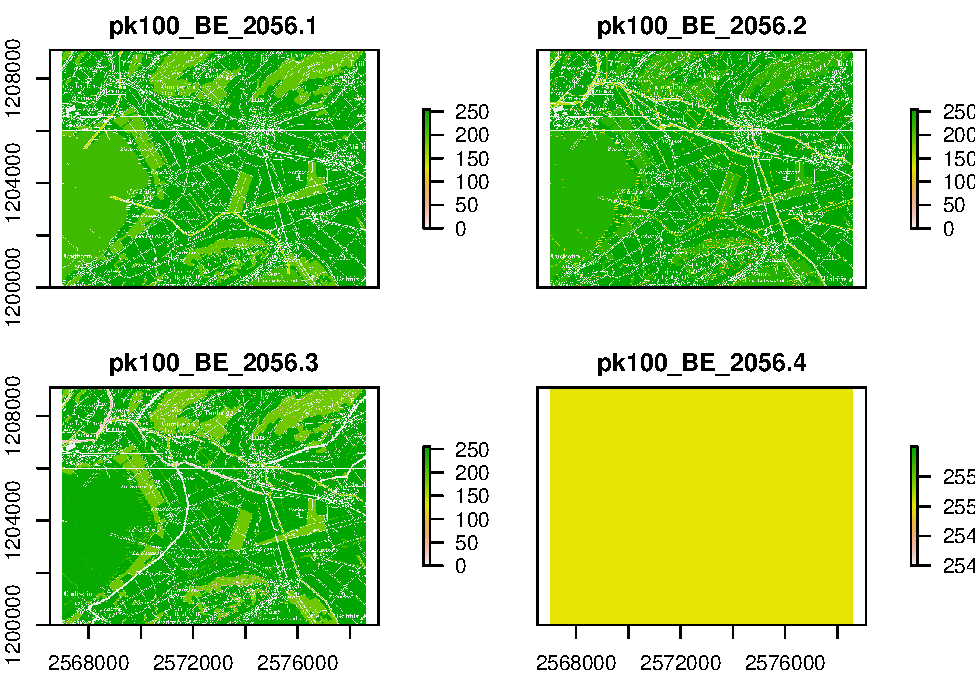
\includegraphics{_main_files/figure-latex/import raster data-1.pdf}

\begin{Shaded}
\begin{Highlighting}[]
\CommentTok{\# remove the 4th layer}
\NormalTok{pk100\_BE }\OtherTok{\textless{}{-}} \FunctionTok{subset}\NormalTok{(pk100\_BE, }\DecValTok{1}\SpecialCharTok{:}\DecValTok{3}\NormalTok{)}
\FunctionTok{plot}\NormalTok{(pk100\_BE)}
\end{Highlighting}
\end{Shaded}

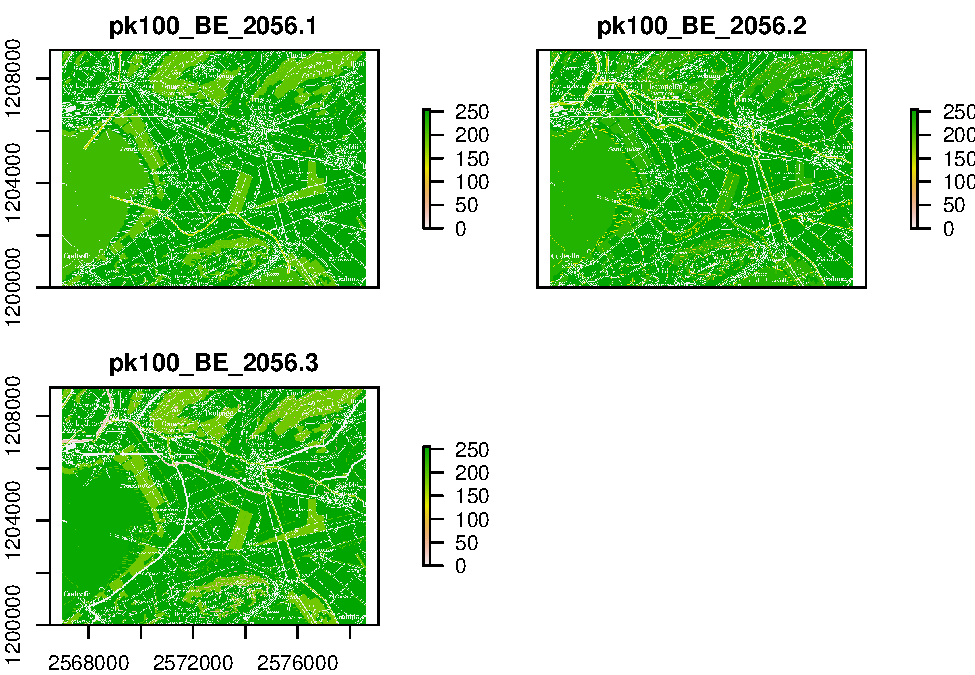
\includegraphics{_main_files/figure-latex/import raster data-2.pdf}

\hypertarget{task-6-adding-a-background-map}{%
\section{Task 6: Adding a background map}\label{task-6-adding-a-background-map}}

\begin{verbatim}
## stars object downsampled to 1129 by 886 cells. See tm_shape manual (argument raster.downsample)
\end{verbatim}

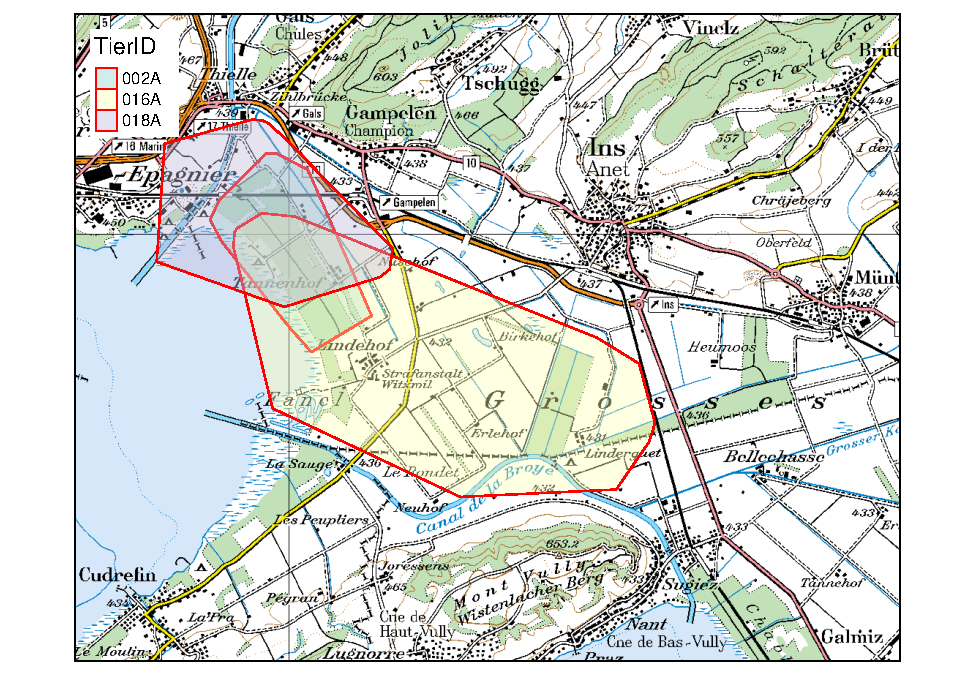
\includegraphics{_main_files/figure-latex/background map-1.pdf}

\end{document}
